\documentclass[pdflatex]{sn-jnl}
 \renewcommand{\textfraction}{.002}
\renewcommand{\floatpagefraction}{.995}
\setcounter{totalnumber}{5}
\renewcommand{\topfraction}{.995}

\usepackage[numbers,square]{natbib}
\bibliographystyle{spbasic_u}

\usepackage[noend,ruled,vlined]{algorithm2e}
\newcommand\mycommfont[1]{\footnotesize\ttfamily{#1}}
\SetCommentSty{mycommfont}


\usepackage{graphicx}%
\usepackage{multirow}%
\usepackage{amsmath,amssymb,amsfonts}%
\usepackage{amsthm}%
\usepackage{mathrsfs}%
\usepackage[title]{appendix}%
\usepackage{xcolor}%
\usepackage{textcomp}%
\usepackage{manyfoot}%
\usepackage{booktabs}%
\usepackage{placeins}
\usepackage{listings}%
\usepackage{mathtools}
\usepackage{subcaption}
\usepackage{xr}
\usepackage{bm}
%% CUSTOM PACKAGES
%\usepackage[linesnumbered,ruled,vlined]{algorithm2e}
\usepackage{hyperref}
\usepackage{array}
\usepackage{tabularx}
\usepackage{tikz}
\usetikzlibrary{shapes.geometric}
%\usetikzlibrary{3d,perspective}
%\usetikzlibrary{shapes.geometric, arrows.meta, positioning}
\usepackage{booktabs} % For better table lines
\usepackage[version=4]{mhchem} 
\usepackage{enumitem}
\usepackage{algorithm2e}
%\usepackage{arydshln}

%%%%%%%%%%%%%%%%%%%%%%%%%%%%%%%%%%%%%%%%%%%%%%%%%%%%%%%%%%%%%%%%%%%%%%%%%%%

%% as per the requirement new theorem styles can be included as shown below
\theoremstyle{thmstyleone}%
\newtheorem{theorem}{Theorem}%  meant for continuous numbers
\newtheorem{corollary}[theorem]{Corollary}% 
\newtheorem{proposition}[theorem]{Proposition}%
\newtheorem{lemma}[theorem]{Lemma}% 
\newtheorem{conjecture}[theorem]{Conjecture}%
\newtheorem{observation}[theorem]{Observation}%
%
\makeatletter
\newtheoremstyle{examplesty}% Numbered
{18pt plus2pt minus1pt}% Space above
{18pt plus2pt minus1pt}% Space below
{\normalfont}% Body font
{0pt}% Indent amount
{\bfseries}% Theorem head font
{.}% Punctuation after theorem head
{.5em}% Space after theorem headi
{\thmname{#1}\thmnumber{\@ifnotempty{#1}{ }{#2}}%
  \thmnote{ {\the\thm@notefont(#3)}}}% Theorem head spec (can be left empty, meaning `normal')
\makeatother
\theoremstyle{examplesty}%
\newtheorem{example}{Example}%
%\newtheorem{remark}{Remark}%
%
\theoremstyle{thmstylethree}%
\newtheorem{definition}[theorem]{Definition}%

\newenvironment{mainitem}[2]{\medskip\par\noindent%
  \textbf{#1~M\ref{#2}.}}{\par}


%%%%% SOME LOW LEVEL STUFF NEEDED FOR SPECIAL SYMBOLS
\makeatletter
\def\moverlay{\mathpalette\mov@rlay}
\def\mov@rlay#1#2{\leavevmode\vtop{%
    \baselineskip\z@skip \lineskiplimit-\maxdimen
    \ialign{\hfil$\m@th#1##$\hfil\cr#2\crcr}}}
\newcommand{\charfusion}[3][\mathord]{
  #1{\ifx#1\mathop\vphantom{#2}\fi
    \mathpalette\mov@rlay{#2\cr#3}
  }
  \ifx#1\mathop\expandafter\displaylimits\fi}
\DeclareRobustCommand\bigop[1]{%
  \mathop{\vphantom{\sum}\mathpalette\bigop@{#1}}\slimits@
}
\newcommand{\bigop@}[2]{%
  \vcenter{%
    \sbox\z@{$#1\sum$}%
    \hbox{\resizebox{\ifx#1\displaystyle.9\fi\dimexpr\ht\z@+\dp\z@}{!}{$\m@th#2$
}}%
  }%
}
\makeatother
%%%%% END LOWLEVEL USER DEFINITION

\newcommand{\cupdot}{\charfusion[\mathbin]{\cup}{\cdot}}
\DeclareMathOperator{\bigcupdot}{\charfusion[\mathop]{\bigcup}{\cdot}}
% \DeclareMathOperator{\Aut}{Aut}
% \DeclareMathOperator{\orb}{orb}
\newcommand{\whatever}{\mbox{\,.\,}}
\newcommand{\king}{K}
\newcommand{\queen}{\mathbf{Q}}
\newcommand{\prince}{\mathbf{P}}
\newcommand{\food}{\ensuremath{\mathbf{F}}}
\newcommand{\SM}{\mathbb{S}}
\newcommand{\closure}[2]{\mathscr{C}_{#1}(#2)}
\newcommand{\cl}[0]{c}
\newcommand{\CR}[0]{\mathcal{R}}
\newcommand{\C}[1]{\mathit{#1}}
\newcommand{\FR}[0]{\mathbf{R}}
%\newcommand{\F}[1]{\mathbf{#1}}
\newcommand{\fr}[0]{\mathbf{r}}
\newcommand{\net}[1]{\hat{#1}}
\newcommand{\RAF}[0]{\mathbf{R}'}
\newcommand{\PO}[0]{d}
\newcommand{\POR}[0]{\mathscr{R}}
\newcommand{\POX}[0]{\mathscr{X}}
\newcommand{\cat}{\mathbf{C}}
\newcommand{\sgen}{g}
\newcommand{\rgen}{\gamma}
\newcommand{\ceducts}{\mathcal{E}}
\newcommand{\cproducts}{\mathcal{P}}
\newcommand{\feducts}{\mathbf{E}}
\newcommand{\fproducts}{\mathbf{P}}
\newcommand{\ORCID}[1]{}
\DeclareMathOperator{\suck}{succ}
\newcommand{\Code}[1]{\texttt{\upshape{#1}}}
\newcommand{\pfad}[0]{\ensuremath{\mathbf{P}}}
\newcommand{\stack}[0]{\ensuremath{\mathbf{T}}}
\newcommand{\child}{\pmb{\kappa}}

\definecolor{middlegreen}{RGB}{0,128,0}
\definecolor{royalpurple}{RGB}{85,26,139}
\newcommand{\NEW}[1]{\begingroup\color{blue}#1\endgroup}
\newcommand{\TODO}[1]{\begingroup\color{red}#1\endgroup}
\newcommand{\PFS}[1]{\begingroup\color{blue}#1\endgroup}
\newcommand{\holy}[1]{\begingroup\color{royalpurple}#1\endgroup}
\newcommand{\TG}[1]{\begingroup\color{green}#1\endgroup}
\newcommand{\NV}[1]{\begingroup\color{teal}#1\endgroup}
\newcommand{\OLD}[1]{\begingroup\tiny\color{gray}#1\endgroup}

% Linenumbers for debugging
\usepackage{lineno}
\linenumbers
\raggedbottom

%%%%%%%%%%%%%%%%%%%%%%%%%%%%%%%%%%%%%%%%%%%%%%%%%%%%%%%%%%%%%%%%%%%
%%%%%%%%%%%%%%%%%%%%%%%%%%%%%%%%%%%%%%%%%%%%%%%%%%%%%%%%%%%%%%%%%%%
%%%%%%%%%%%%%%%%%%%%%%%%%%%%%%%%%%%%%%%%%%%%%%%%%%%%%%%%%%%%%%%%%%%

\begin{document}

\title{RAF-Cores: Deadwood} 


\maketitle


\vspace{6pt}
\begin{lemma}
	Every $\fr\in \RAF$ has at least one reactant (F-reactant or F-catalyst) that is not in $\food$. For 
	$\fr\in \RAF: \rgen(\fr)=1$, this is an F-catalyst.
\end{lemma}
\begin{proof}
	 Assume this is not the case for an $\fr\in \RAF$. Then $\{\fr\}$ is a RAF which contradicts minimality
	 and non-triviality of $\RAF$.
\end{proof}

Since all food molecules are absent in $\queen''$, it contains an elementary circuit since all vertices have an 
in-degree greater than zero \cite{bang-jensen_digraphs_2002}. Since $\queen''\subseteq \queen'$ we obtain:
\vspace{6pt}
\begin{corollary}
	The graphs $\queen'$ and $\queen''$ contain an elementary circuit. 
\end{corollary}
\vspace{6pt}

In \cite{steel_minimal_2013} this was already shown for the reaction graph, but not for the bipartite graph. For minimal RAFs, this result 
can be strengthened to the statement that every reaction in $\queen'$ and $\queen''$ is located on an elementary circuit. We start by 
showing that each first-generation reaction is located on an elementary circuit. To this end, we define the descendants and ascendants 
of a vertex $v$ in a graph in the following way

\begin{equation}
	\begin{split}
		D(v) & \coloneqq \{u \in V \ | \text{ exists a path } P=(v,\ldots, u)  \} \\
		A(v) & \coloneqq \{u \in V \ | \text{ exists a path } P=(u,\ldots, v)  \} \\
	\end{split}
\end{equation}

\begin{lemma}
	Let $\RAF$ be a minimal, non-trivial RAF. Then every first-generation reaction 
	is located on an elementary circuit that is not a digon in $\queen'$ and $\queen''$.
\end{lemma}
\begin{proof}
	We start with $\queen''$ and assume this is not the case. Then there is a first-generation 
	reaction $\fr_1$, that has no incoming edges. Thus, all F-reactants and all F-catalysts are 
	in $\food$. Then $\{\fr_1\}$ is a RAF which directly contradicts that $\RAF$ is a non-trivial 
	and minimal RAF. Then $\fr_1$ has an incoming edge, and since $\rgen(\fr_1)=1$ all 
	F-reactants are in $\food$, which implies that there is $c_1\in X(\cat(\fr_1)): c_1\notin \food$
	and there by $(c_1,\fr_1),(\fr_1,c_1) \in E(\queen')$. However, this is a digon and if $c_1\notin 
	D(\fr_1)$ then $c_1\in D(\fr_2)$ for some $\fr_2: \rgen(\fr_2)=1$, thus $\fr_1\in D(\fr_2)$. Now, we apply 
	the same argument as above for $\fr_2$, i.e., there has to be a $c_2 \in X(\cat(\fr_2)): c_2\notin \food$
	otherwise $\{\fr_2\}$ is a RAF contradicting the minimality and non-triviality of $\RAF$. 
	Thus there is $c_2\in \cat_{\fr_2}: c_2\notin F$. Then there is an $\fr_3: \rgen(\fr_3)=1: c_2\in D(\fr_3)$ 
	We repeat the arguments until we reach an $\fr_l$ such that $\fr_l=\fr_k$ for some $k<l$, thus we reach 
	an F-reaction again, which is guaranteed since $\RAF$ is finite. Then all reactions $r_k, \ldots, r_{l-1}$ 
	are located on an elementary circuit. If $l>1$ then $\RAF'\coloneqq \RAF\setminus (D(\fr_1)\cup\{\fr_1\})$ 
	is non-empty since it contains the reactions $\fr_k,\ldots, \fr_{l-1}$ and on top a RAF.
	To see this, assume it is not the case. First, $\RAF'\subseteq \RAF$ implies that is reflexively autocatalytic. Then 
	there is again a reaction $\fr'\in \RAF'$ for which a reactant or a catalyst $x$ is not in $\closure{\RAF'}{\food}$. 
	Since $x\in \closure{\RAF}{\food}$ then $x\in D(\fr_1)$. Then $\fr'\in D(\fr_1)$, a contradiction. Thus, $\RAF'$ is
	a RAF, and $\RAF$ was not minimal. Adding the food molecules does not change the argument, thus the 
	statement also holds for $\queen''$.
\end{proof}
\vspace{6pt}

\holy{RG rewriting upto here}

We now extend this result to all residual reaction vertices.

\vspace{6pt}
\begin{lemma}\label{lem:elemCirc}
	Let $(X,R, \cat)$ be a catalyzed network with food-set $F$, and $\RAF$ be a minimal, non-trivial RAF. Then 
	every $r\in \RAF$ is part of an elementary circuit that is not a digon in $G$ and $H$.
\end{lemma}
\begin{proof}
	Again, we start with the graph $H$. We know that each $r_1\in \POR^1_{\RAF}(F)$ is 
	is located on an elementary circuit. Assume now there is a reaction $r\in \RAF$ that is 
	not located on an elementary circuit. We now show that $\RAF' \coloneqq \RAF\setminus 
	(R(D(r))\cup \{r\}$ is a RAF. First, we observe that $\RAF'\neq \emptyset$, since $\POR^1_{\RAF}(F) 
	\subseteq \RAF'$. Otherwise, $r$ would be located on an elementary circuit. Therefore, 
	assume $\RAF'$ is not a $\RAF$. Since $\RAF$ is reflexively autocatalytic and 
	$\RAF'\subseteq \RAF$, $\RAF'$ is reflexively autocatalytic. Then, there is a reaction 
	$r'\in \RAF'$ for which a reactant or a catalyst $x\in X(H)$ with $s^-_{xr'}>0$ it holds that 
	$x\notin \closure{\RAF'}(F)$. Since $x\in \closure{\RAF}(F)$ is a product of some reaction 
	$r''\in R(D(R'))\cup \{r'\}$. However, then $r''\in R(D(R'))\cup \{r'\}$, which is a contradiction. 
	Thus, $\RAF'$ is a RAF and therefore $\RAF$ was not minimal. Adding the food molecules 
	to $H$ does not change the arguments, thus the result also holds for $G$. 		
\end{proof}
\vspace{6pt}

We say that two elementary circuits $C_1, C_2$ are 1-connected from $C_1$ to $C_2$ if there are vertices $u\in V(C_1)$ 
and $v\in V(C_2)$ such that there is a path $P_{uv}$ connecting them. Since elementary circuits are strongly connected, 
if $C_1$ and $C_2$ are 1-connected from $C_1$ to $C_2$ there is a path $P_{uv}$ connecting any two vertices $u\in V(C_1)$ 
and $v\in V(C_2)$. We say two elementary circuits are strongly connected if they are 1-connected from $C_1$ to $C_2$ and 
from $C_2$ to $C_1$.
\vspace{6pt}
\begin{lemma}\label{lem:strElCirc}
	Let $(X,R, \cat)$ be a catalyzed network with food-set $F$, and $\RAF$ a minimal, non-trivial RAF. Any two elementary circuits $C_1,C_2$ 
	in $G \ (H)$ are strongly connected. 
\end{lemma}
	\begin{proof}
		We start again with $G$ and reaction vertices in $\POR^1_{\RAF}(F)$. Assume the trivial case $|\POR^1_{\RAF}(F)|=1$. According to 
		Lemma~\ref{lem:elemCirc}, $r^*\in \POR^1_{\RAF}(F)$ is located on an elementary circuit $C^*$. Assume there is an elementary
		circuit $C\neq C^*$ such that $C^*$ is not strongly-connected with $C$. Since $G$ is weakly-connected and $|\POR^1_{\RAF}(F)|=1$, 
		$C^*$ is $1$-connected to $C$. If $C$ is not $1$-connected to $C^*$ then $\RAF\setminus R(C)$ is a RAF thus $\RAF$ not minimal. 
		Now assume that $|\POR^1_{\RAF}(F)|>1$ and let $r_1,r_2\in \POR^1_{\RAF}(F)$. Then $r_1,r_2$ are located on two elementary circuits
		$C_1$ and $C_2$. If $C_1=C_2$, there is nothing to show. Thus, assume $C_1\neq C_2$. If $C_1$ is not 1-connected to $C_2$ and 
		vice versa, then $\RAF\setminus R(C_2)$ is a RAF and $\RAF\setminus R(C_2)$ is a RAF which contradicts minimality of $\RAF$. So 
		assume that $C_1$ is 1-connected to $C_2$, but $C_2$ is not $1$-connected to $C_1$. Then $\RAF\setminus R(C_2)$ is a $\RAF$ 
		contradicting minimality. Substituting the roles of $C_1$ and $C_2$ yields that $C_1$ and $C_2$ are strongly connected. Together
		with the trivial case, this implies that any two elementary circuits are strongly connected. The same arguments hold for $H$.
	\end{proof}
\vspace{6pt}

The graph $H$ does not contain any $f\in F$, thus any vertex in $H$ has at least one incoming edge. By Lemma~\ref{lem:elemCirc}, 
any reaction vertex is located on an elementary circuit. Since elementary circuits are pairwisely strongly connected, species vertices
are either located on an elementary circuit themselves, or they connect two elementary circuits, $C_1$ and $C_2$, i.e., reactants of
a reaction of $C_1$ and a product of a reaction of $C_2$. Thus, such vertices are thereby directly located themselves on an elementary 
circuit. Nevertheless, $H$ might contain species that are only products but never reactants, and thus have no outgoing edges, as the 
following example illustrates. 
\begin{figure}[h]
	\centering
	\begin{minipage}[c]{0.3\textwidth}
		\begin{equation}
			\begin{split}
				r_1& : f \overset{x_1}{\longrightarrow} x_2 \\
				r_2& : x_2 \overset{x_2}{\longrightarrow} x_1 + x_3
			\end{split}
		\end{equation}
	\end{minipage}%
	\hfill%
	\begin{minipage}[c]{0.23\textwidth}
		\centering
		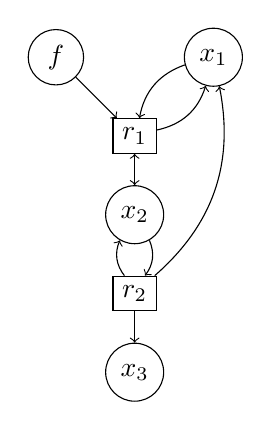
\begin{tikzpicture}
			\node[draw, circle] (f) at (0,0) {$f$};
			\node[draw, circle] (x1) at (2,0) {$x_1$};	
			\node[draw, circle] (x2) at (1,-2) {$x_2$};
			\node[draw, circle] (x3) at (1,-4) {$x_3$};
		
			\node[draw, rectangle] (r1) at (1,-1) {$r_1$};
			\node[draw, rectangle] (r2) at (1,-3) {$r_2$};
		
			\draw[->] (f) to (r1);
			\draw[->] (x1) to [bend right = 30] (r1);
			\draw[->] (r1) to [bend right = 30] (x1);
			\draw[->] (r1) to (x2);
			\draw[->] (x2) to [bend left = 30](r2);
			\draw[->] (r2) to [bend left = 30](x2);
			\draw[->] (x2) to (r1);
			\draw[->] (r2) to (x3);
			\draw[->] (r2) to [bend right = 30] (x1);
		\end{tikzpicture}	
	\end{minipage}%
	\hfill%
	\begin{minipage}[c]{0.23\textwidth}
		\centering
		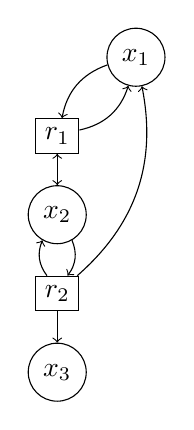
\begin{tikzpicture}
			\node[draw, circle] (x1) at (2,0) {$x_1$};	
			\node[draw, circle] (x2) at (1,-2) {$x_2$};
			\node[draw, circle] (x3) at (1,-4) {$x_3$};
		
			\node[draw, rectangle] (r1) at (1,-1) {$r_1$};
			\node[draw, rectangle] (r2) at (1,-3) {$r_2$};
		
			\draw[->] (x1) to [bend right = 30] (r1);
			\draw[->] (r1) to [bend right = 30] (x1);
			\draw[->] (r1) to (x2);
			\draw[->] (x2) to [bend left = 30](r2);
			\draw[->] (r2) to [bend left = 30](x2);
			\draw[->] (x2) to (r1);
			\draw[->] (r2) to (x3);
			\draw[->] (r2) to [bend right = 30] (x1);
		\end{tikzpicture}	
	\end{minipage}%
	\hfill%
	\begin{minipage}[c]{0.23\textwidth}
		\centering
		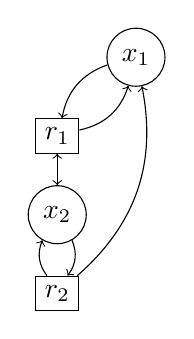
\begin{tikzpicture}
			\node[draw, circle] (x1) at (2,0) {$x_1$};	
			\node[draw, circle] (x2) at (1,-2) {$x_2$};
		
			\node[draw, rectangle] (r1) at (1,-1) {$r_1$};
			\node[draw, rectangle] (r2) at (1,-3) {$r_2$};
		
			\draw[->] (x1) to [bend right = 30] (r1);
			\draw[->] (r1) to [bend right = 30] (x1);
			\draw[->] (r1) to (x2);
			\draw[->] (x2) to [bend left = 30](r2);
			\draw[->] (r2) to [bend left = 30](x2);
			\draw[->] (x2) to (r1);
			\draw[->] (r2) to [bend right = 30] (x1);
		\end{tikzpicture}	
	\end{minipage}
	\caption{A minimal RAF $\RAF$ \textit{(left)} with its directed K\"onig graph represnetation 
	$G\coloneqq \king[\closure{\RAF}{F}, \RAF]$  \textit{(middle left)}, $H\coloneqq \king[\closure{\RAF}{F} 
	\setminus F, \RAF]$ \textit{(middle right)}, and $L\coloneqq H[V(H) \setminus W, \RAF], W 
	\coloneqq \{x\in \closure{\RAF}{F} \ | \ \nexists r \in \RAF \text{ s.t. } s^-_{xr}>0\}$ \textit{(right)}.}
	\label{fig:}
\end{figure}
\FloatBarrier

Indeed, $\{r_1,r_2\}$ is a RAF w.r.t. to $F$. Nevertheless, $x_3$ is never consumed by any reaction. Naturally, any strictly positive reaction 
vector yields a net increase in the concentration of such species, which motivates to consider the graph $H$ without those vertices. In addition, 
these species are never located on an elementary circuit, and we obtain that Lemma~\ref{lem:strElCirc} holds if these species are removed.
\vspace{6pt}
\begin{corollary}\label{lem:strElCirc}
	Let $(X,R, \cat)$ be a catalyzed network with food-set $F$, and $\RAF$ a minimal, non-trivial RAF. Any two elementary circuits $C_1,C_2$ 
	in $L\coloneqq H[V(H)\setminus W]$ with $W\coloneqq \{x\in \closure{\RAF}{F} \ | \ \nexists r \in \RAF \text{ s.t. } s^-_{xr}>0\}$ are strongly connected. 
\end{corollary}
\vspace{6pt}
For brevity of presentation, we let 
\begin{equation}\label{eq:graphL}
	L\coloneqq H[V(H]\setminus W], W\coloneqq \{x\in \closure{\RAF}{F} \ | \ \nexists r \in \RAF \text{ s.t. } s^-_{xr}>0\} 
\end{equation}
in the following. If $\RAF$ is composed of a single reaction, then $L$ is a singleton, i.e., the very reaction vertex of $\RAF$. 
We may therefore directly conclude:

\end{document}